\documentclass[12pt, titlepage]{article}

\usepackage{fullpage}
\usepackage[round]{natbib}
\usepackage{multirow}
\usepackage{booktabs}
\usepackage{tabularx}
\usepackage{graphicx}
\usepackage{xcolor}
\usepackage{url}
\usepackage{caption}
%\usepackage{geometry}

\usepackage{xr}
\usepackage{hyperref}
\usepackage[numbib,nottoc]{tocbibind}

\hypersetup{
 bookmarks=true,   % show bookmarks bar?
 colorlinks=true,  % false: boxed links; true: coloured links
 linkcolor=red,   % color of internal links (change box color 
%with linkbordercolor)
 citecolor=black!40,  % color of links to bibliography
 filecolor=magenta,  % color of file links
 urlcolor=cyan   % color of external links
}

%% Comments

\usepackage{color}

\newif\ifcomments\commentstrue

\ifcomments
\newcommand{\authornote}[3]{\textcolor{#1}{[#3 ---#2]}}
\newcommand{\todo}[1]{\textcolor{red}{[TODO: #1]}}
\else
\newcommand{\authornote}[3]{}
\newcommand{\todo}[1]{}
\fi

\newcommand{\wss}[1]{\authornote{blue}{SS}{#1}}
\newcommand{\an}[1]{\authornote{magenta}{Author}{#1}}


\newcommand{\progname}{SSP}

\newcounter{acnum}
\newcommand{\actheacnum}{AC\theacnum}
\newcommand{\acref}[1]{AC\ref{#1}}

\newcounter{ucnum}
\newcommand{\uctheucnum}{UC\theucnum}
\newcommand{\uref}[1]{UC\ref{#1}}

\newcounter{mnum}
\newcommand{\mthemnum}{M\themnum}
\newcommand{\mref}[1]{M\ref{#1}}

%\newgeometry{margin=2cm}

% define "struts", as suggested by Claudio Beccari in
%    a piece in TeX and TUG News, Vol. 2, 1993.
\newcommand{\Tstrut}{\rule{0pt}{2.6ex}}         % = `top' strut

\externaldocument[SRS-]{SRS_SSP}
\externaldocument[MIS-]{MIS_SSP}

\begin{document}

\title{Module Guide for Slope Stability Analysis Program} 
\author{Henry Frankis and Brooks MacLachlan}
\date{\today}

\maketitle

\pagenumbering{roman}

\section{Revision History}

\begin{tabularx}{\textwidth}{p{3cm}p{2cm}X}
	\toprule {\bf Date} & {\bf Version} & {\bf Notes}\\
	\midrule
	31/10/2018 & 1.0 & Initial template updates\\
	\bottomrule
\end{tabularx}

\newpage

\section{Reference Material}
This section records information for easy reference.
\subsection{Abbreviations and Acronyms}

\renewcommand{\arraystretch}{1.2}
\begin{tabular}{l l} 
	\toprule		
	\textbf{Symbol} & \textbf{Description}\\
	\midrule 
	AC & Anticipated Change\\
	DAG & Directed Acyclic Graph \\
	M & Module \\
	MG & Module Guide \\
	OS & Operating System \\
	R & Requirement\\
	RFEM & Rigid Finite Element \\
	SC & Scientific Computing \\
	SRS & Software Requirements Specification\\
	\progname & Slope Stability Analysis Program\\
	UC & Unlikely Change \\
	\bottomrule
\end{tabular}\\

\bmac{This section is not on the template but I think that it should be since 
this document introduces many new acronyms}

\newpage

\tableofcontents

\listoftables

\listoffigures

\newpage

\pagenumbering{arabic}

\section{Introduction}

\hspace{3ex}Decomposing a system into modules is a commonly accepted
approach to developing software.  A module is a work assignment for a
programmer or programming team~\citep{ParnasEtAl1984}.  In the best
practices for Scientific Computing (SC), \citet{WilsonEtAl2013} advise a
modular design, but are silent on the criteria to use to decompose the
software into modules.  We advocate a decomposition based on the
principle of information hiding~\citep{Parnas1972a}.  This principle
supports design for change, because the ``secrets'' that each module
hides represent likely future changes.  Design for change is valuable
in SC, where modifications are frequent, especially during initial
development as the solution space is explored.

Our design follows the rules laid out by \citet{ParnasEtAl1984}, as follows:
\begin{itemize}  
\item System details that are likely to change independently should be
  the secrets of separate modules.
\item Any other program that requires information stored in a module's
  data structures must obtain it by calling access programs belonging
  to that module.
\end{itemize}

In a rational design process, the Module Guide (MG) is developed after 
completing the Software Requirements Specification (SRS) 
\citep{ParnasEtAl1984}. The MG specifies the modular
structure of the system and is intended to allow both designers and
maintainers to easily identify the parts of the software.  The
potential readers of this document are as follows:

\begin{itemize}
\item New project members: This document can be a guide for a new
  project member to easily understand the overall structure and
  quickly find the relevant modules they are searching for.
\item Maintainers: The hierarchical structure of the module guide
  improves the maintainers' understanding when they need to make
  changes to the system. It is important for a maintainer to update
  the relevant sections of the document after changes have been made.
\item Designers: Once the module guide has been written, it can be
  used to check for consistency, feasibility, and flexibility. Designers can 
  verify the system in various ways, such as consistency among modules, 
  feasibility of the decomposition, and flexibility of the design.
\end{itemize}

The rest of the document is organized as follows. Section
\ref{SecChange} lists the anticipated and unlikely changes of the
software requirements. Section \ref{SecMH} summarizes the module
decomposition that was constructed according to the likely
changes. Section \ref{SecConnection} specifies the connections between
the software requirements and the modules. Section \ref{SecMD} gives a
detailed description of the modules. Section \ref{SecTM} includes two
traceability matrices. One checks the completeness of the design
against the requirements provided in the SRS. The other shows the
relation between anticipated changes and the modules. Section
\ref{SecUse} describes the use relation between modules.

\section{Anticipated and Unlikely Changes} \label{SecChange}

\hspace{3ex}This section lists possible changes to the
system. According to the likeliness of the change, the possible
changes are classified into two categories. Anticipated changes are
listed in Section \ref{SecAchange}, and unlikely changes are listed in
Section \ref{SecUchange}.

\subsection{Anticipated Changes} \label{SecAchange}

\hspace{3ex}Anticipated changes are the source of the information that
is to be hidden inside the modules. Ideally, changing one of the
anticipated changes will only require changing the one module that
hides the associated decision. The approach adapted here is called
design for change. Anticipated changes are numbered by \textbf{AC}
followed by a number.

\begin{description}
\item[AC\refstepcounter{acnum}\theacnum \label{AC_hardware}:] The
  specific hardware on which the software is running.
\item[AC\refstepcounter{acnum}\theacnum \label{AC_Control}:] The
  algorithm for the overall operation procedure of the program.
\item[AC\refstepcounter{acnum}\theacnum \label{AC_input}:] The format
  of the initial input data.
\item[AC\refstepcounter{acnum}\theacnum \label{AC_output}:] The format
  of the final output data.
\item[AC\refstepcounter{acnum}\theacnum \label{AC_GenAlg}:] Algorithm
  for determining the critical slip surface.
\item[AC\refstepcounter{acnum}\theacnum \label{AC_Kin}:] Criteria for
  a slip surface to be considered physically realistic/ kinematically
  admissible.
\item[AC\refstepcounter{acnum}\theacnum \label{AC_Slicer}:] The
  algorithm for creating the slice points for slip surface analysis.
\item[AC\refstepcounter{acnum}\theacnum \label{AC_FSweight}:] The
  weighting scheme for comparing slip surfaces factors of safety.
\item[AC\refstepcounter{acnum}\theacnum \label{AC_MP}:] The
  algorithm for implementation of the Morgenstern Price Solver.
\item[AC\refstepcounter{acnum}\theacnum \label{AC_RFEM}:] The
  algorithm for implementation of the RFEM Solver.
\item[AC\refstepcounter{acnum}\theacnum \label{AC_PropSorter}:] The
  algorithm for assigning soil properties to slices.
\item[AC\refstepcounter{acnum}\theacnum \label{AC_Array}:] The
  implementation for the sequence (array) data structure.
\item[AC\refstepcounter{acnum}\theacnum \label{AC_Rand}:] The method
  of generating pseudo-random numbers.
\item[AC\refstepcounter{acnum}\theacnum \label{AC_Plot}:] The method
  of displaying the final output.
\end{description}


\subsection{Unlikely Changes} \label{SecUchange}

\hspace{3ex}The module design should be as general as
possible. However, a general system is more complex. Sometimes this
complexity is not necessary. Fixing some design decisions at the
system architecture stage can simplify the software design. If these
decision should later need to be changed, then many parts of the
design will potentially need to be modified. Hence, it is not intended
that these decisions will be changed.  As an example, the model is
assumed to follow the definition in the SRS.  If a new model is used,
this will mean a change to the input format, fit parameters module,
control, and output format modules. Unlikely changes are numbered by \textbf{UC} followed by a number.

\begin{description}
\item [\refstepcounter{ucnum}UC\theucnum \label{UC_IO}:] Input/Output
  devices (Input: File and/or Keyboard, Output: File, Memory, and/or
  Screen).
\item [\refstepcounter{ucnum}UC\theucnum \label{UC_inputsource}:]
  There will always be a source of input data external to the
  software.
\item [\refstepcounter{ucnum}UC\theucnum \label{UC_output}:] Output
  data are displayed to the output device.
\end{description}


\section{Module Hierarchy} \label{SecMH}

\hspace{3ex}This section provides an overview of the module
design. Modules are summarized in a hierarchy decomposed by secrets
in Table~\ref{Table:Decomp}. The modules listed below are the modules
that will actually be implemented. Modules are numbered by \textbf{M}
followed by a number.

\begin{description}
\item [\refstepcounter{mnum} \mthemnum \label{mHH}:] Hardware-Hiding
  Module
\item [\refstepcounter{mnum} \mthemnum \label{mControl}:] Control
  Module
\item [\refstepcounter{mnum} \mthemnum \label{mInput}:] Input Format
  Module
\item [\refstepcounter{mnum} \mthemnum \label{mOutput}:] Output Format
  Module
\item [\refstepcounter{mnum} \mthemnum \label{mGenAlg}:] Genetic
  Algorithm Module
\item [\refstepcounter{mnum} \mthemnum \label{mKinAdm}:] Kinematic
  Admissibility Module
\item [\refstepcounter{mnum} \mthemnum \label{mSlipSlicer}:] Slip
  Slicer Module
\item [\refstepcounter{mnum} \mthemnum \label{mSlipWeight}:] Slip
  Weighting Module
\item [\refstepcounter{mnum} \mthemnum \label{mMorgPrice}:]
  Morgenstern Price Solver Module
\item [\refstepcounter{mnum} \mthemnum \label{mRFEM}:] Rigid Finite
  Element Method Solver Module
\item [\refstepcounter{mnum} \mthemnum \label{mSliceProperty}:] Slice
  Property Sorter Module
\item [\refstepcounter{mnum} \mthemnum \label{mArrayOps}:] Sequence
  Data Structure Module
\item [\refstepcounter{mnum} \mthemnum \label{mRandNum}:] Random
  Number Generator Module
\item [\refstepcounter{mnum} \mthemnum \label{mPlot}:] Plotting
  Module
\end{description}

Note that \mref{mHH} is a commonly used module and is already
implemented by the operating system.

\begin{table}[h!]
\centering
\begin{tabular}{p{0.3\textwidth} p{0.6\textwidth} }
\toprule
\textbf{Level 1} & \textbf{Level 2} \\
\midrule

{Hardware-Hiding Module} & ~ \\
\midrule

\multirow{8}{0.3\textwidth}{Behaviour-Hiding Module} &
Control Module \\
& Input Format Module \\
& Output Format Module \\
& Genetic Algorithm Module \\
& Kinematic Admissibility Module \\
& Slip Slicer Module \\
& Slip Weighting Module \\
& Morgenstern Price Solver Module \\
& RFEM Solver Module \\
& Slice Property Sorter Module \\
\midrule

\multirow{3}{0.3\textwidth}{Software Decision Module} &
Sequence Data Structure Module \\
& Random Number Generating Module \\
& Plotting Module \\
\bottomrule

\end{tabular}
\caption{Module Hierarchy}
\label{Table:Decomp}
\end{table}

\section{Connection Between Requirements and Design} \label{SecConnection}

\hspace{3ex}The design of the system is intended to satisfy the
requirements developed in the SRS. In this stage, the system is
decomposed into modules. The connection between requirements and
modules is listed in Table~\ref{Table:Req}. The program implements two
distinct solution methods of calculating the factor of safety of the
slope, the Morgenstern Price method and the Rigid Finite Element
(RFEM) method, both developed in the SRS. The Morgenstern Price solver
is implemented by \mref{mMorgPrice}, further information on the
Morgenstern Price algorithm can be found in \cite{ZhuEtAl2005}. The RFEM solver
is implemented by \mref{mRFEM}, further information on the RFEM
algorithm can be found in \cite{StolleGuo}. The critical slip identification
goal (G2,IM4 in SRS) is implemented by use of a genetic algorithm
\mref{mGenAlg}, further information on use of a genetic algorithm in
relation to a slope stability problem can be found in \cite{LiEtAl}.


\section{Module Decomposition} \label{SecMD}

\hspace{3ex}Modules are decomposed according to the principle of
``information hiding'' proposed by \citet{ParnasEtAl1984}. The
\emph{Secrets} field in a module decomposition is a brief statement of
the design decision hidden by the module. The \emph{Services} field
specifies \emph{what} the module will do without documenting
\emph{how} to do it. For each module, a suggestion for the
implementing software is given under the \emph{Implemented By}
title. If the entry is \emph{OS}, this means that the module is
provided by the operating system or by standard programming language
libraries. \emph{\progname} means the module will be implemented by
the \progname. Only the leaf modules in the hierarchy have
to be implemented. If a dash (\emph{--}) is shown, this means that the
module is not a leaf and will not have to be implemented. Whether or
not this module is implemented depends on the programming language
selected.

\subsection{Hardware-Hiding Modules (\mref{mHH})}

\begin{description}
\item[Secrets:]The data structure and algorithm used to implement the
  virtual hardware.
\item[Services:]Serves as a virtual hardware used by the rest of the
  system. This module provides the interface between the hardware and
  the software. So, the system can use it to display outputs or to
  accept inputs.
\item[Implemented By:] OS
\end{description}

\subsection{Behaviour-Hiding Module}

\begin{description}
\item[Secrets:]The contents of the required behaviors.
\item[Services:]Includes programs that provide externally visible
  behaviors of the system as specified in the software requirements
  specification (SRS) documents. This module serves as a communication
  layer between the hardware-hiding module and the software decision
  module. The programs in this module will need to change if there are
  changes in the SRS.
\item[Implemented By:] --
\end{description}

\subsubsection{Control Module (\mref{mControl})}

\begin{description}
\item[Secrets:] The algorithm for coordinating the running of the
  program.
\item[Services:] Provides the main program.
\item[Implemented By:] \progname
\end{description}


\subsubsection{Input Format Module (\mref{mInput})}

\begin{description}
\item[Secrets:]The format and structure of the input data.
\item[Services:] Reads the input data from an input file, and/or
  prompted command line inputs. Input data includes the x,y
  coordinates of the slope, with a set of coordinates for each
  layer. For each layer its soil properties of effective angle of
  friction, effective cohesion, dry unit weight, saturated unit
  weight, elastic modulus, and Poisson's ratio are stored in vectors
  of soil properties. If a piezometric surface exists in the slope,
  its coordinates and the unit weight of water are also included in
  the input. Lastly an expected range for the entrance and exit points
  of the critical slip surface are inputted.
\item[Implemented By:] \progname
\end{description}

\subsubsection{Output Format Module (\mref{mOutput})}

\begin{description}
\item[Secrets:] The format and structure of the output data.
\item[Services:] Outputs the results of the calculations, including
  the factor of safety for the critical slip calculated by the
  Morgenstern Price Module (\mref{mMorgPrice}) and Rigid Finite
  Element Method Module (\mref{mRFEM}), and a plot of the critical
  slip surface on the slope geometry, with the showing the element
  displacements as calculated by the RFEM Module
\item[Implemented By:] \progname
\end{description} 


\subsubsection{Genetic Algorithm Module (\mref{mGenAlg})}

\begin{description}
\item[Secrets:] Algorithm to identify the slip surface that has the
  minimum factor of safety, based on the inputs.
\item[Services:] Searches the slope for the critical slip surface with
  the minimum factor of safety 
\item[Implemented By:] \progname
\end{description}


\subsubsection{Kinematic Admissibility Module (\mref{mKinAdm})}

\begin{description}
\item[Secrets:] Algorithm to determine if a given slip surface passes
  or fails a set of admissibility criteria.
\item[Services:] Some slip surfaces are physically unlikely or
  impossible to occur in a slip surface, such as slip surfaces
  containing sharp angles, or going above the slope surface. Ensures
  randomly generated or mutated slopes from the Genetic Algorithm
  Module (\mref{mGenAlg}) are physically possible according to the
  criteria of the Kinematic Admissibility Module.
\item[Implemented By:] \progname
\end{description} 


\subsubsection{Slip Slicer Module (\mref{mSlipSlicer})}

\begin{description}
\item[Secrets:] Algorithm to determine the coordinates of where the
  slip surface interslice nodes occur.
\item[Services:] When preparing a slip surface for analysis by the
  Morgenstern Price Module (\mref{mMorgPrice}) or the RFEM Module
  (\mref{mRFEM}), the x-coordinates defining the boundaries of the
  slices are identified and stored in a vector.
\item[Implemented By:] \progname
\end{description} 

\subsubsection{Slip Weighting Module (\mref{mSlipWeight})}

\begin{description}
\item[Secrets:] The weighting for each slip surface in a set of slip
  surfaces, based on each slip surfaces factor of safety.
\item[Services:] Weights a set of slip surfaces generated by the
  Genetic Algorithm Module (\mref{mGenAlg}) based on their factors of
  safety. A slip surface with a low factor of safety will have a high
  weight as it is more likely to be or to lead to generation of the
  critical slip surface.
\item[Implemented By:] \progname
\end{description} 

\subsubsection{Morgenstern Price Solver Module (\mref{mMorgPrice})}

\begin{description}
\item[Secrets:] The factor of safety of a given slip surface.
\item[Services:] Calculates the factor of safety of a given slip
  surface, through implementation of a Morgenstern Price slope
  stability analysis method.
\item[Implemented By:] \progname
\end{description} 


\subsubsection{RFEM Solver Module (\mref{mRFEM})}

\begin{description}
\item[Secrets:] The algorithm to perform a Rigid Finite Element Method
  analysis of the slope.
\item[Services:] Calculate the global factor of safety, local slice
  factors of safety, and local slice displacements of a given slip
  surface under given conditions, through implementation of a rigid
  finite element slope stability analysis method.
\item[Implemented By:] \progname
\end{description}

\subsubsection{Slice Property Sorter Module (\mref{mSliceProperty})}
\begin{description}
\item[Secrets:] Algorithm to assigns soil properties to slices based
  on the location of the slice with respect to the different soil
  layers.
\item[Services:] When performing slip analysis with the RFEM Solver
  Module (\mref{mRFEM}) or Morgenstern Price Module
  (\mref{mMorgPrice}), the base and interslice surfaces of each slice
  in the analysis requires a soil constant. Slice Property Sorter
  Module identifies which soil layer the surface is in to assign
  properties from that soil layer, and uses a weighting scheme when
  the surface crosses multiple soil layers.
\item[Implemented By:] \progname
\end{description} 


\subsection{Software Decision Module}

\begin{description}
\item[Secrets:] The design decision based on mathematical theorems,
  physical facts, or programming considerations. The secrets of this
  module are \emph{not} described in the SRS.
\item[Services:] Includes a data structure and algorithms used in the
  system that do not provide direct interaction with the user.
\item[Implemented By:] --
\end{description}


\subsubsection{Sequence Data Structure Module (\mref{mArrayOps})}

\begin{description}
\item[Secrets:] The data structure for a sequence data type.
\item[Services:] Provides array manipulation, including building an
  array, accessing a specific entry, slicing an array etc.
\item[Implemented By:] Matlab
\end{description}


\subsubsection{Random Number Generator Module (\mref{mRandNum})}

\begin{description}
\item[Secrets:] Pseudo-random numbers between 0 and 1.
\item[Services:] Randomly produces numbers between 0 and 1, using a
  chaotic function with an external seed. Used when generating slip
  surfaces in the Genetic Algorithm Module \mref{mGenAlg}.
\item[Implemented By:] Matlab
\end{description}


\subsubsection{Plotting Module (\mref{mPlot})}

\begin{description}
\item[Secrets:] The data structures and algorithms for plotting data
  graphically.
\item[Services:] Provides a plot function.
\item[Implemented By:] Matlab
\end{description}

\section{Traceability Matrix} \label{SecTM}

\hspace{3ex}This section shows two traceability matrices: between the
modules and the requirements Table~\ref{Table:Req} and between the
modules and the anticipated changes Table~\ref{Table:AC}.

\begin{table}[h!]
\centering
\begin{tabular}{ll}
\toprule
\textbf{Req.} & \textbf{Modules}\\
\midrule
R1 & \mref{mControl} \mref{mInput} \mref{mArrayOps}\\
R2 & \mref{mGenAlg} \mref{mRandNum} \mref{mArrayOps}\\
R3 & \mref{mKinAdm} \mref{mArrayOps}\\
R4 & \mref{mGenAlg} \mref{mSlipSlicer} \mref{mArrayOps}\\
R5 & \mref{mMorgPrice} \mref{mArrayOps}\\
R6 & \mref{mSlipWeight} \mref{mArrayOps}\\
R7 & \mref{mGenAlg} \mref{mRandNum} \mref{mArrayOps}\\
R8 & \mref{mGenAlg} \mref{mArrayOps}\\
R9 & \mref{mControl} \mref{mOutput} \mref{mSlipSlicer} \mref{mArrayOps}\\
R10 & \mref{mOutput} \mref{mMorgPrice} \mref{mRFEM} \mref{mArrayOps}\\
R11 & \mref{mOutput} \mref{mPlot}\\
\bottomrule
\end{tabular}
\caption{Trace Between Requirements and Modules}
\label{Table:Req}
\end{table}

\begin{table}[h!]
\centering
\begin{tabular}{ll}
\toprule
\textbf{Req.} & \textbf{Modules}\\
\midrule
\acref{AC_hardware} & \mref{mHH}\\
\acref{AC_Control} & \mref{mControl}\\
\acref{AC_input} & \mref{mInput}\\
\acref{AC_output}& \mref{mOutput}\\
\acref{AC_GenAlg}& \mref{mGenAlg}\\
\acref{AC_Kin}& \mref{mKinAdm}\\
\acref{AC_Slicer} & \mref{mSlipSlicer}\\
\acref{AC_FSweight}& \mref{mSlipWeight}\\
\acref{AC_MP} & \mref{mMorgPrice}\\
\acref{AC_RFEM} & \mref{mRFEM}\\
\acref{AC_PropSorter}& \mref{mSliceProperty}\\
\acref{AC_Array} & \mref{mArrayOps}\\
\acref{AC_Rand} & \mref{mRandNum}\\
\acref{AC_Plot} & \mref{mPlot}\\
\bottomrule
\end{tabular}
\caption{Trace Between Anticipated Changes and Modules}
\label{Table:AC}
\end{table}

\section{Use Hierarchy Between Modules} \label{SecUse}

\hspace{3ex}In this section, the uses hierarchy between modules is
provided. \cite{Parnas1978} said of two programs A and B that A {\em
  uses} B if correct execution of B may be necessary for A to complete
the task described in its specification. That is, A {\em uses} B if
there exist situations in which the correct functioning of A depends
upon the availability of a correct implementation of B. 
Figure~\ref{Fig_Use} illustrates the use hierarchy between the modules. The
graph is a directed acyclic graph (DAG). Each level of the hierarchy
offers a testable and usable subset of the system, and modules in the
higher level of the hierarchy are essentially simpler because they use
modules from the lower levels.

% ------ %
\begin{figure}[h!]
\begin{center}
{
 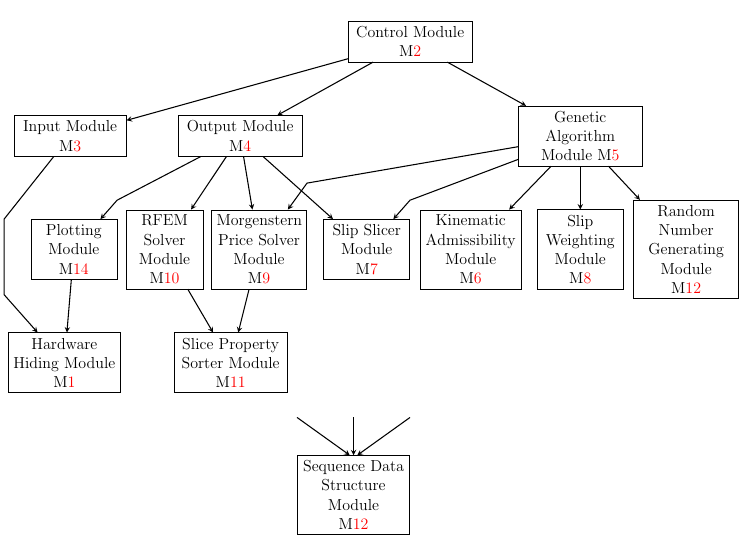
\includegraphics[width=1.1\textwidth]{UseHierarchyDiagram3.png}
}
\caption{Use Hierarchy Diagram}
\label{Fig_Use}
\end{center}
\end{figure}
% ------ %
~\newpage
\bibliographystyle {plainnat}
\bibliography {../../../refs/References}

\end{document}
